\RequirePackage{luatex85}
\documentclass[11pt]{scrreprt}

\usepackage{fontspec}
\usepackage{xcolor}
\usepackage{csquotes}
\usepackage{marginnote}
\usepackage{tikz}
\usepackage{geometry}
\usepackage[ngerman]{babel}
\defaultfontfeatures{Ligatures=TeX}
% Set sans serif font to Calibri
\setsansfont{Calibri}
% Set serifed font to Cambria
\setmainfont{Cambria}
% Define light and dark Microsoft blue colours
\definecolor{MSBlue}{rgb}{.204,.353,.541}
\definecolor{MSLightBlue}{rgb}{.31,.506,.741}
\addtokomafont{section}{\color{MSBlue}}
\addtokomafont{subsection}{\color{MSLightBlue}}


\usepackage[backend=biber,style=alphabetic,hyperref=true,backref=true,block=none,url=false,isbn=false,doi=false,maxcitenames=3,maxbibnames=100]{biblatex}
\addbibresource{references.bib}

\title{Die bunte Welt der Farbstoffe}
\author{Lukas Braun}
\publishers{
\includegraphics[width=5cm]{logo.jpg} \\ Descartes Gymnasium Neuburg a. d. Donau}
\subject{Chemie}
\subtitle{W-Seminar -- Chemisch Kochen}
%TODO Abgabedatum
\date{21. Dezember 2012}

\geometry{
	a4paper,
	left=30mm,
	right=20mm,
	top=25mm,
	bottom=25mm
}

\usepackage[onehalfspacing]{setspace}
\emergencystretch=.5em


\begin{document}

\maketitle
\clearpage

\tableofcontents
\clearpage
\chapter{Definitionen von Farben}
Um Farben sehen zu können, wird Licht benötigt, denn wie das Sprichwort sagt sind Nachts alle Katzen grau. Dies lässt sich auf Atomebene recht einfach erklären: Hierfür müssen zunächst Elektronen innerhalb der Atome durch die Zufuhr von Wärmeenergie angeregt werden und dadurch auf eine höhere Energiestufe (= höhere Geschwindigkeit und größere Entfernung zum Atomkern)  gehoben werden. Da dieser Zustand relativ energiereich und damit instabil ist, fällt das Elektron auf sein ursprüngliches Energieniveau zurück. Die daraus resultierende Energiedifferenz kann, abhängig vom Molekülbau, als Wärmestrahlung oder als Lichtstrahlung (=Photonenstrahlung) abgegeben werden. Kommt das entstandene Licht wiederum auf einen anderen Stoff an, so geschieht dort das gleiche. Jeder Stoff kann jedoch nur Licht bestimmter Wellenlängen absorbieren. Die restlichen Wellenlängen werden reflektiert, und durch additive Mischung dieser Wellenlängen resultiert die für den Menschen erscheinende Eigenfarbe des Stoffes.
%\begin{figure}[ht!]
%	\centering
%	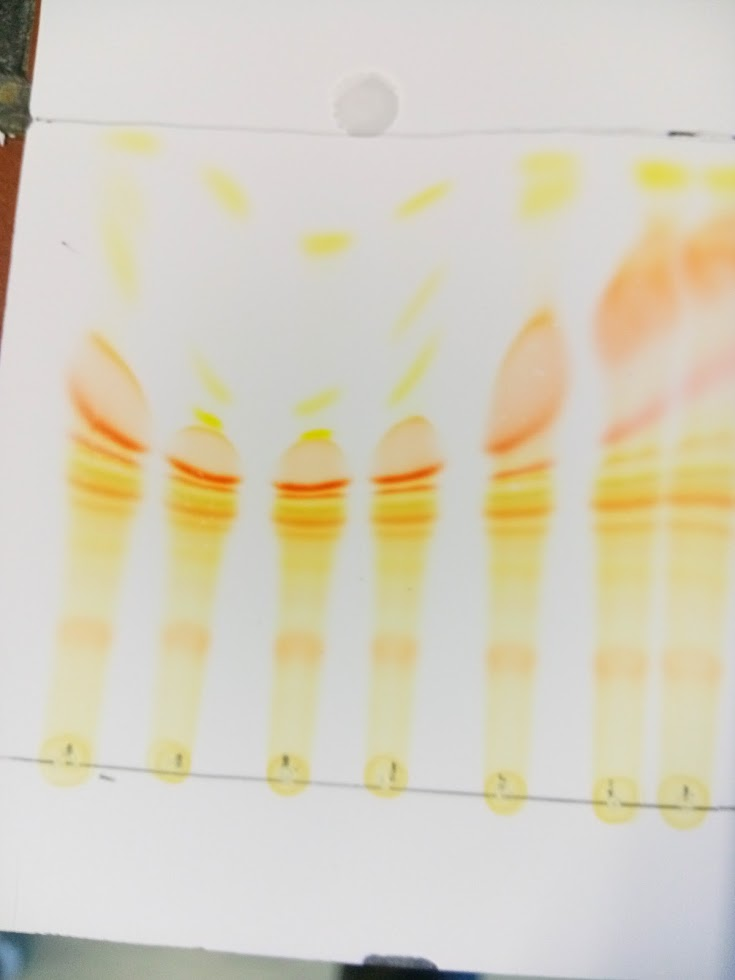
\includegraphics[width=\textwidth]{paprika.jpg}
%	\caption{Entstehung der Farbigkeit eines stoffes}
%	\label{img:Reflektion und Addition von Licht}
%\end{figure}n
\chapter{E-Nummern}

E-Nummern sind toll \cite[S. 12]{Schobert.2007}. \cite[j]{Schobert.2007}



\chapter{Farbstoffextraktion}
Dünnschichtchromatografie gilt als eine einfache Farbstofftrennmethode, bei der auf eine stationäre Phase (hier: Kieselgel auf einer Kunststoffplatte und Aluminiumoxid auf einem Aluminiumblech) die zu untersuchende Substanz in gelöster Form mithilfe von Glaskapillaren punktförmig aufgetragen wird.  Daraufhin stellt man die mobile Phase (auch Lauf- oder Fließmittel genannt) aus verschiedenen unterschiedlich polaren\footnote{Die Polarität entscheidet zudem unter anderem die Wasserlöslichkeit} Lösungsmitteln her. Die Trennung der Farbstoffe basiert auf die unterschiedlichen Löslichkeit in den verwendeten Lösungsmitteln.
Die unterschiedlichen zwischenmolekularen Wechselwirkungen, wie Dipol"=Dipol"=Wechselwirkungen oder Van-der-Waals-Wechselwirkungen der Lösungsmittel ermöglichen ein breiteres Spektrum an lösbaren Stoffen mit dem gleichen Gemisch. Sie entstehen durch Ladungstrennung innerhalb der Molekülen (Dipol-Ionen Bindungen) oder durch unterschiedliche Partialladungen \footnote{Auch Teilladungen genannt}, das heißt dort ist die Wahrscheinlichkeit erhöht auf Ladungstrennungen zu treffen. Dieser Effekt wird durch die Adsorption(Anreicherung einer Flüssigkeit an der Oberfläche eine Festkörpers ), Verteilung des gelösten Stoffes oder den Siebeffekten(bei dem, wie bei einem Küchensieb kleinere Stoffe hindurch gelangen und größere die feste Phase nicht, oder langsamer nach oben hin durchdringen können)
Ziel der Dünnschichtchromatografie ist der stoffspezifische Rf- Wert (\enquote{Ratio of front}). Er gibt das Verhältnis der Laufmittelfront (Höhe des Laufmittels) und der Fließhöhe des Stoffes. Dieser Wert hängt von dem Laufmittelgemisch und dessen Konzentration, dem Trägermaterial, der Versuchstemperatur und der chemischen Struktur der Substanz ab. Zudem ist die Dampfsättigung innerhalb einer einfachen Entwicklungskammer recht unregelmäßig. Dies ist der Grund für die relativ schlechte Vergleichbarkeit von RF-Werten
 

\section{Paprika}
Oft ist Paprika im örtlichen Supermarkt in den Farben Rot, Grün und Gelb erhältlich. Deshalb klingt es auch nur vernünftig, anzunehmen, dass in einer Paprikafrucht mehrere verschiedenen Farbstoffe enthalten sind, je nach Farbe in einer jeweils anderen Konzentration. In einer Paprikaschote überwiegen im unreifen Zustand der grüne Blattfarbstoff Chlorophyll. Während des Reifungsprozesses wird jedoch das Chlorophyll abgebaut und es erscheint die gelbe bis tiefrote Farbe der Carotinoide. Der Großteil dieser Carotinoide sind rot.\footnote{Ein Beispiel hierfür ist Capsanthin}.
Diese Carotinoide schützen das Photosynthese treibende Chlorophyll vor Photooxidation. Hierbei geht das durch Licht angeregte Chlorophyllmolekül in den Triplettzustand über. In diesem hochreaktionären Zustand kann Energie auf umliegenden Sauerstoff übergehen, der daraufhin mit dem Chlorophyllmolekül reagiert, wodurch dieser abgebaut wird.
Diese Photooxidation wird durch die Carotinoide unterbunden.
Zudem wird durch Carotinoide das Absorptionsspektrum des Organismus im grünen bis blauen Farbbereich erweitert, sodass noch mehr (Licht-)Energie der Photosynthese zur Verfügung steht.

%\begin{figure}[ht!]
%	\centering
%	\includegraphics[width=\textwidth]{bild.png}
%	\caption{Das ist ein Bild}
%	\label{img:chromatographie_1}
%\end{figure}

\begin{figure}[ht!]
\centering
\begin{tikzpicture}
\node[anchor=south west,inner sep=0] (image) at (0,0,0) {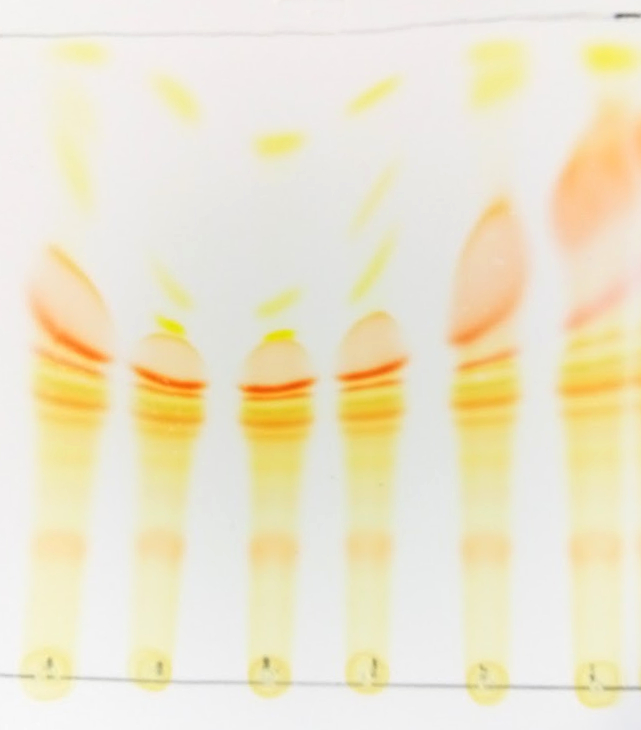
\includegraphics[width=0.5\textwidth]{paprika_editiert.jpg}};
\begin{scope}[x={(image.south east)},y={(image.north west)}]
%% next four lines will help you to locate the point needed by forming a grid. comment these four lines in the final picture.↓
%      \draw[help lines,xstep=.1,ystep=.1] (0,0) grid (1,1);
%        \draw[help lines,xstep=.05,ystep=.05] (0,0) grid (1,1);
%        \foreach \x in {0,1,...,9} { \node [anchor=north] at (\x/10,0) {0.\x}; }
%        \foreach \y in {0,1,...,9} { \node [anchor=east] at (0,\y/10) {0.\y};}
%% upto here↑
\draw[-latex,thick] (0.95,0.98 ) -- +(1cm,0.2cm)node[anchor=west] {Fließmittelfront};
\draw[-latex,thick] (0.94,0.75) -- +(2cm,0)node[anchor=west] {Substanz};
\draw[-latex,thick] (0.94,0.06) -- +(2cm,0)node[anchor=west] {Startpunkt};

\end{scope}
\end{tikzpicture}
	\caption{Dünnschichtchromatographie von Paprikasaft}
	\label{img:paprika}
\end{figure}

%TODO Weiterschreiben

Wie man in Abbildung \ref{img:paprika}
\section{gefärbte Schokoladenlinsen}
Wie bereits geschrieben, werden Lebensmittelfarben vor allem in industriell gefertigten Gütern verwendet, um bei den Verbrauchern eine bessere oder andere Qualität vorzutäuschen. So werden vor allem Süßigkeiten mit möglichst glänzenden und kräftigen Lebensmittelfarben gefärbt. Auch sind die Schokoladenlinsen nicht auf natürliche Weise unterschiedlich farbig, sondern werden mit Gemischen aus 3 Stoffen (Chinolingelb, Karmin (rot) und Patentblau) die 4 verschiedenen Farben erstellt. Um auf die 4 Farben zu kommen muss zusätzlich Chinolingelb mit Karmin(ergibt Orange), und Karmin mit Patentblau(ergibt braun) gemischt werden.
Dieses Ergebnis kann mithilfe einer Dünnschichtchromatografie nachvollzogen werden.

\begin{figure}[ht!]
	\centering
	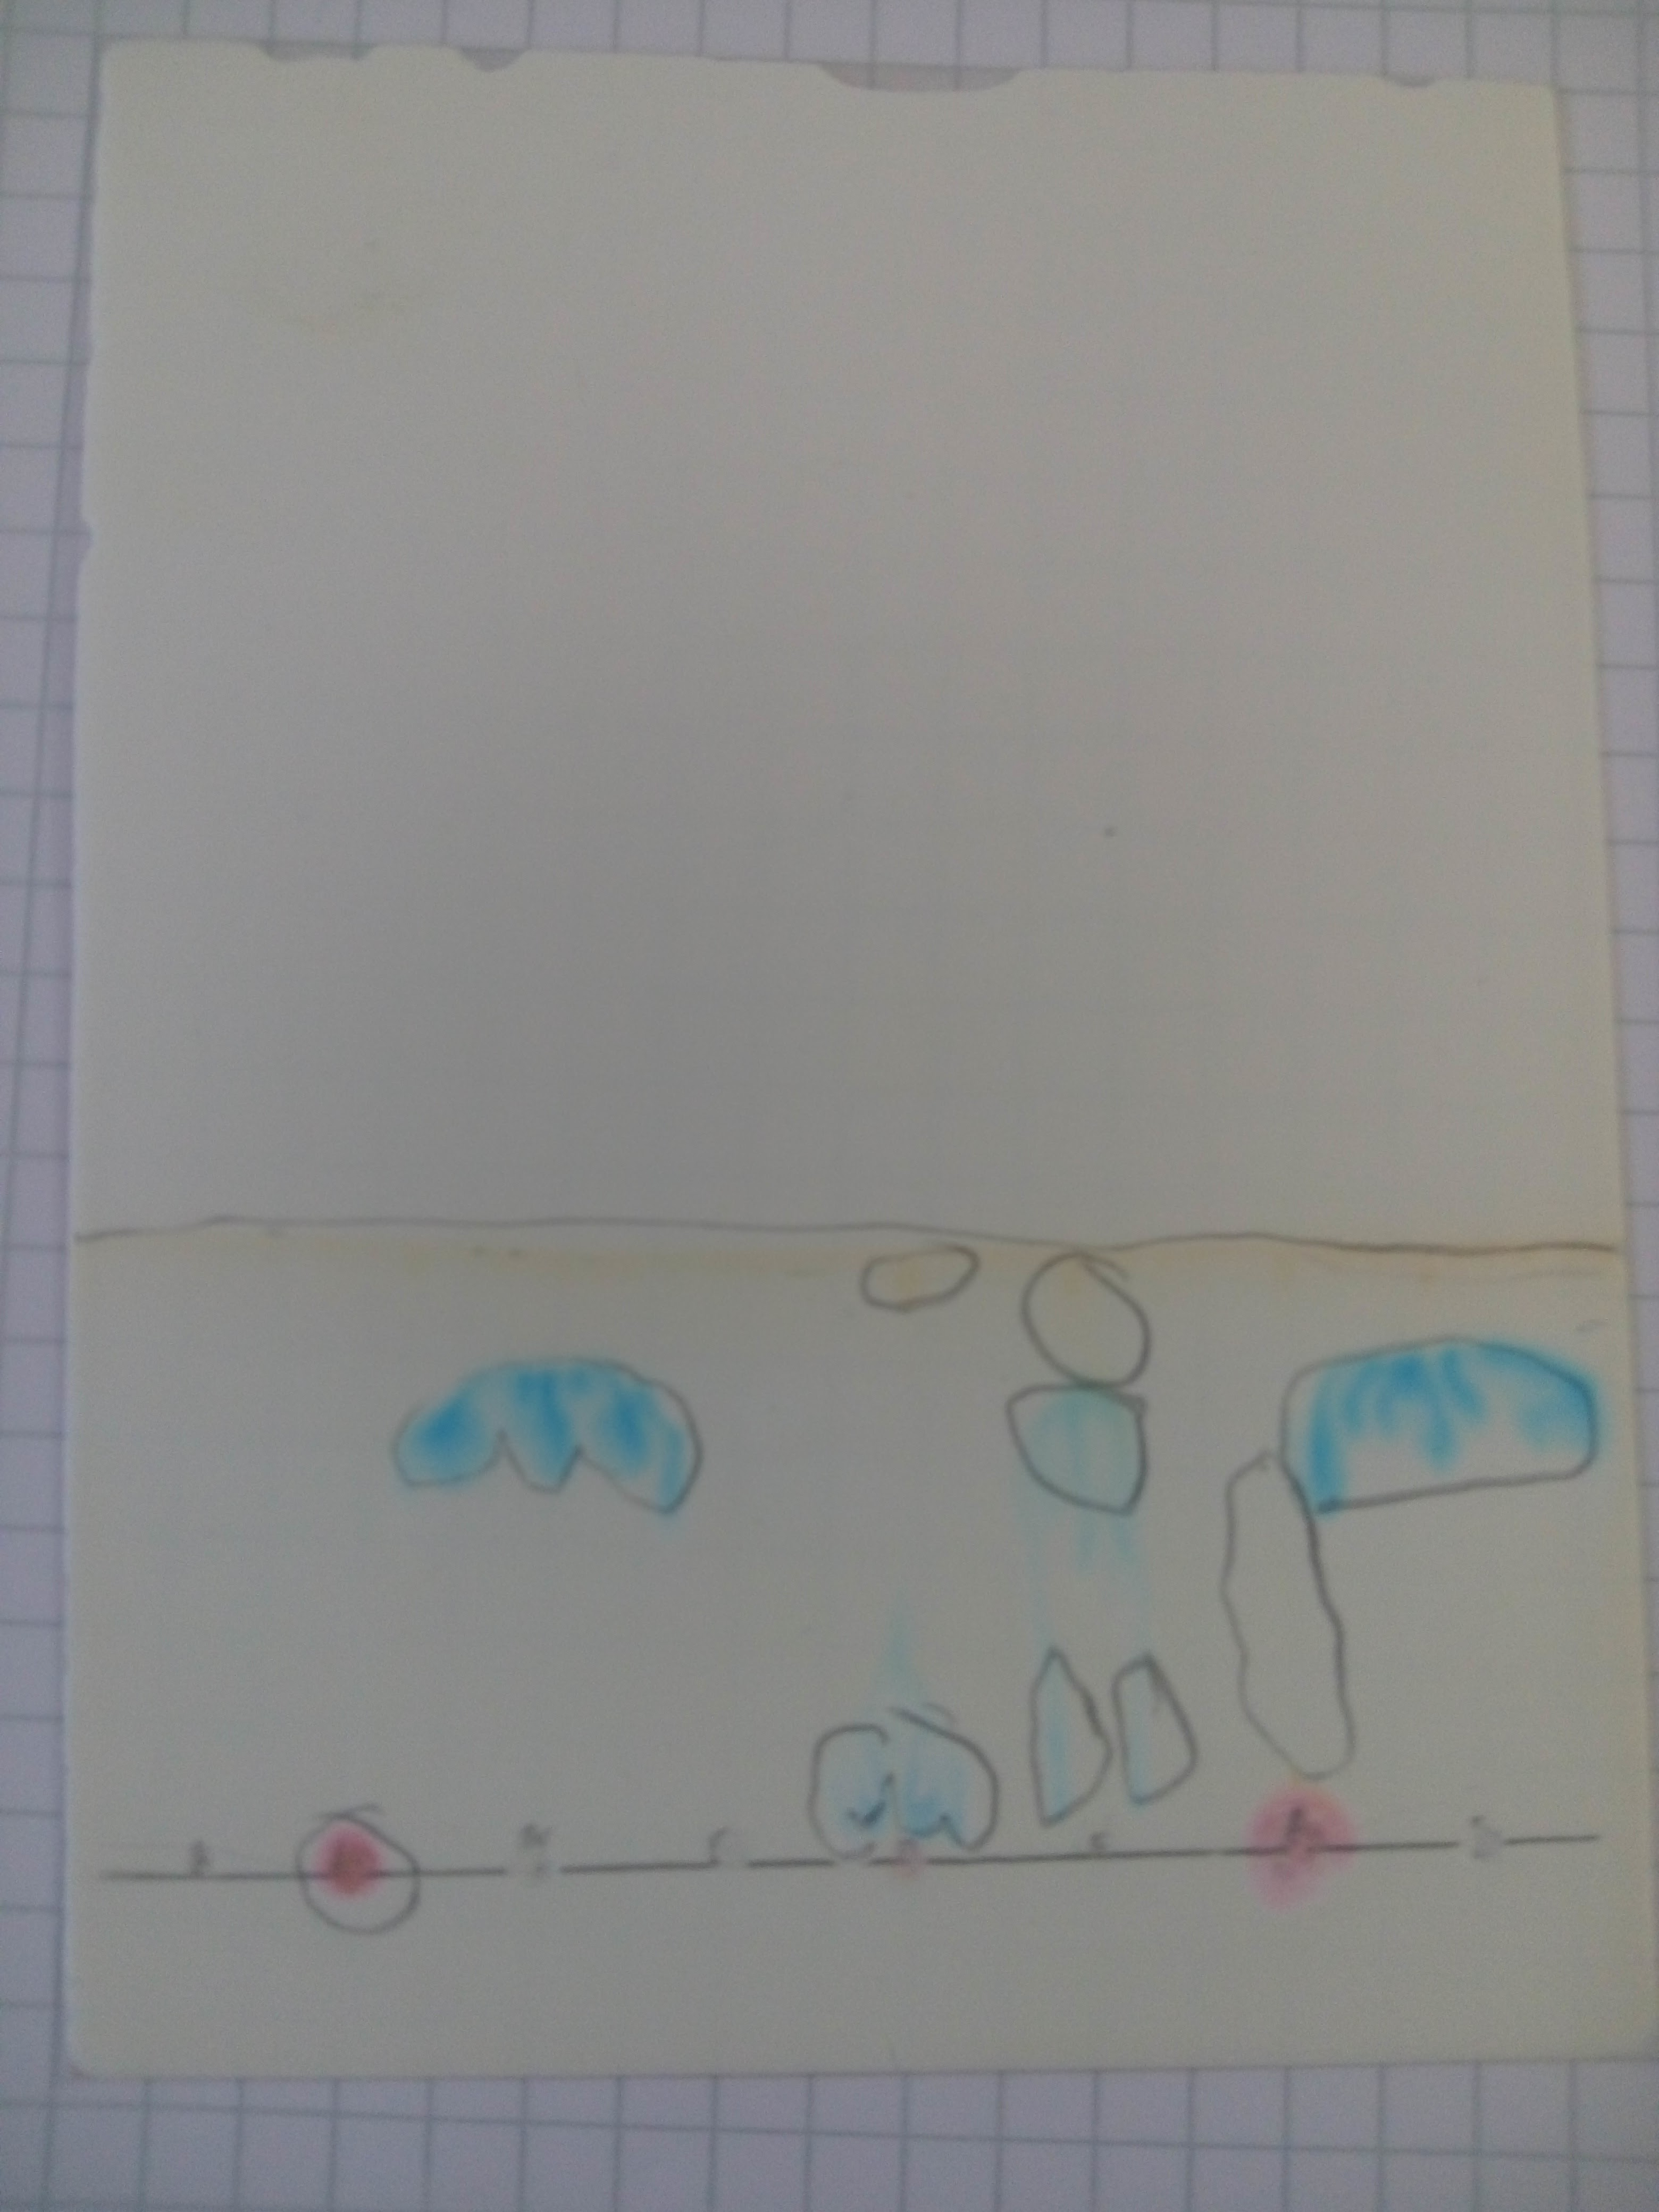
\includegraphics[width=\textwidth]{kieselgel.jpg}
	\caption{Dünnschichtchromatografie mit Schokolinsen (Kieselgelplatte)}
	\label{img: Kieselgel}
\end{figure}n
Nach einer Laufzeit von 20 Minuten ist das Laufmittelgemisch, bestehend aus Ethylacetat, Propan-1-ol und Wasser (Verhältniss: 10:60:30) cm an der Kieselgelplatte hochgeflossen.


\printbibliography


\chapter*{Eigenständigkeitserklärung}

Ich habe diese Seminararbeit ohne fremde Hilfe angefertigt und nur die im Literaturverzeichnis angeführten Quellen und Hilfsmittel benutzt.

\vspace{2\baselineskip}
\noindent Neuburg, den \today
\par\noindent\makebox[2.5in]{} \hfill\makebox[2.0in]{\hrulefill}%
\par\noindent\makebox[2.5in][l]{} \hfill\makebox[2.0in][l]{Lukas Braun}

\end{document}